\documentclass[a4paper,12pt]{article}
%%%%%%%%%%%%%%%%%%%%%%
%%%%%% Packages %%%%%%
%%%%%%%%%%%%%%%%%%%%%%
\usepackage{xeCJK}
\setCJKmainfont{DFKai-SB}
\usepackage[ngerman]{babel}
\usepackage[utf8]{inputenc}
\usepackage[T1]{fontenc}
\usepackage{ifthen}
\usepackage[textwidth=12cm,textheight=22cm,centering]{geometry}
\geometry{top=2.3cm,bottom=2.3cm, left=3cm, right=3cm}
\usepackage[x11names]{xcolor}
\usepackage{background}
\usepackage{tikz}
\usetikzlibrary{backgrounds}
\usepackage{hyperref}
\usepackage{setspace}

%%%%%%%%%%%%%%%%%%%%%%
%%%%% Parameters %%%%%
%%%%%%%%%%%%%%%%%%%%%%
%%%%%%%%%%%%%%%%%%%%%%%%%%%%%%%%%%%
%%%%% Settings for invitation %%%%%
%%%%%%%%%%%%%%%%%%%%%%%%%%%%%%%%%%%

\newcommand\TheName{娟}
\newcommand\TheSecondName{志凯}
\newcommand\Lang{zh}
\newcommand\Gender{f}


\ifthenelse{\equal{\TheSecondName}{}}
    {\newcommand\SingPlur{sg}}
    {\newcommand\SingPlur{pl}}

% Check language
\ifthenelse{\equal{\Lang}{dt}}%
{% German
    \newcommand\TheBGHeading{Einladung}
    \hypersetup{
        pdftitle=Einladung zur Hochzeitsfeier,
        pdfauthor={Bernhard}}
    \newcommand\ClosingPoem{%
    love is the voice under all silences,\\
    the hope which has no opposite in fear;\\
    the strength so strong mere force is feebleness:\\
    the truth more first than sun more last than star
    }
}%
{\ifthenelse{\equal{\Lang}{zh}}%
{% Chinese
    \newcommand\TheBGHeading{喜帖}
    \hypersetup{
        pdftitle=喜帖,
        pdfauthor={本德}}
    \newcommand\ClosingPoem{%
    爱是天时地利的迷信\\
    原来你也在这里
}
}{% English
    \newcommand\TheBGHeading{Invitation}
    \hypersetup{
        pdftitle=Invitation to our wedding party,
        pdfauthor={Bernhard}}
    \newcommand\ClosingPoem{%
    love is the voice under all silences,\\
    the hope which has no opposite in fear;\\
    the strength so strong mere force is feebleness:\\
    the truth more first than sun more last than star
    }
}}
    


%%%%%%%%%%%%%%%%%%%%%%
%%%% New commands %%%%
%%%%%%%%%%%%%%%%%%%%%%
\newcommand*\wb[3]{%
  {\fontsize{#1}{#2}\usefont{U}{webo}{xl}{n}#3}}

\newcommand\RowSepVar[1]{\\[#1]}
\newcommand\RowSep{\RowSepVar{2ex}}

% The page frame
\def\FColor{Firebrick3} % The document font color
% Corners of the page frame
\def\TL{E}
\def\TR{F}
\def\BL{G}
\def\BR{H}

\SetBgColor{\FColor}
\SetBgAngle{0}
\SetBgScale{1}
\SetBgOpacity{1}
\SetBgContents{%
\begin{tikzpicture}
\node at (0.50\paperwidth,12) {\wb{80}{34}{\TL}\rule[60pt]{0.15\paperwidth}{0.4pt}%
  \raisebox{54pt}{%
  \makebox[.3\paperwidth]{\ \fontsize{24}{29}\selectfont\scshape \TheBGHeading }}%
  \rule[60pt]{0.15\paperwidth}{0.4pt}\wb{80}{34}{\TR}};
\node at (1.5,-0.5\paperheight+410) {\rule{0.4pt}{.68\paperheight}};
\node at (19.5,-0.5\paperheight+410) {\rule{0.4pt}{.68\paperheight}};
\node at (0.5\paperwidth,-\paperheight+480) {\wb{80}{34}{\BL}\rule[-10pt]{0.6\paperwidth}{0.4pt}\wb{80}{34}{\BR}} ;
\end{tikzpicture}%
}

% Colorize text
\newcommand*\ColText[1]{\textcolor{\FColor}{#1}}
\newcommand*\SignText[1]{\textcolor{\FColor}{\emph{#1}}}
\newcommand*\Heading[1]{{\fontsize{24}{29}\selectfont\ColText{#1}}\\[0.8em]}
\newcommand*\TabHeading[1]{\multicolumn{2}{@{}l}{{\fontsize{24}{29}\selectfont\ColText{#1}}}\\[0.8em]}

% Switch between single invitees and more than one ('feel free to bring a +1' texts)
\newcommand\SwitchSgPl[2]{%
\ifthenelse{\equal{\SingPlur}{sg}}{#1}{#2}%
}

% Switch for gender of the first name (important for German addressing Liebe vs. Lieber)
\newcommand\SwitchGender[2]{%
\ifthenelse{\equal{\Gender}{f}}{#1}{#2}%
}

\pagestyle{empty}

%%%%%%%%%%%%%%%%%%%%%%
%%%%% Parameters %%%%%
%%%%%%%%%%%%%%%%%%%%%%

\begin{document}
\selectfont\textcolor{Ivory1}{.} \\

% Check language and assign input
\ifthenelse{\equal{\Lang}{dt}}%
{% German
    \Heading{\SwitchGender{Liebe}{Lieber} \emph{\TheName}, \TheSecondName{}}
%
\vfil 
\noindent wir m\"ochten \SwitchSgPl{dich}{euch} herzlich einladen, am

\begin{center}
    \selectfont\ColText{11. November 2011} 
\end{center}
ins
\begin{center}
    \selectfont\ColText{Wirtshaus ``Freude''}\\
    (Musterstr. 11, 81111 M\"unchen)
\end{center}

\noindent zu unserer Hochzeitsfeier zu kommen. 


\vfill{}
\noindent
F\"ur s\"amtliche Fragen und Anregungen \SwitchSgPl{kannst du}{k\"onnt ihr} uns selbstverst\"andlich jederzeit kontaktieren. \SwitchSgPl{Nat\"urlich kannst du jemanden mitbringen. Sag es uns bitte nur rechtzeitig, damit wir planen k\"onnen.}{} 

\vfill

\raggedright
Wir hoffen sehr, dass \SwitchSgPl{du kommen kannst}{ihr kommen k\"onnt}! \RowSepVar{4ex}
\raggedleft{\fontsize{24}{29}\selectfont\SignText{Y \&  B}}

\vfill 

}%
{\ifthenelse{\equal{\Lang}{zh}}%
{% Chinese
    \Heading{亲爱的\emph{\TheName}\SwitchSgPl{:}{、} \TheSecondName\SwitchSgPl{}{:}}
%
\Large
\vfil
\noindent 诚挚邀请你\SwitchSgPl{}{们}参加我们在德国的婚礼,见证我们的幸福。

\vfill

\begin{tabular}[\textwidth]{l l}
时间: & \selectfont\ColText{2011年11月11日}\\
地点: & \selectfont\ColText{慕尼黑, 喜悦餐厅}\\
    & {\normalsize(Musterstra\ss e 11 , 81111 München)}
\end{tabular}

\vfill

\Large

\vfill

\noindent 于我们而言,结婚绝不只是披着白纱的闪耀瞬间或说声``我愿意''。 我们会是关系对等的伴侣,任何一方都无须放弃各自的向往。

\vfill

\raggedright
期待今夏与你\SwitchSgPl{}{们}在慕尼黑相见,分享这份喜悦与甜蜜。\RowSepVar{4ex}
\raggedleft{\fontsize{24}{29}\selectfont\SignText{Y \& 本德}}
\large
\vfill

}{% English
    \Heading{Dear \emph{\TheName}, \TheSecondName{}}
%
\vfil
\noindent we would like to cordially invite you to join our wedding party on 

\begin{center}
    \selectfont\ColText{November 11, 2011}, 
\end{center}
in the
\begin{center}
    \selectfont\ColText{restaurant ``Freude''}\\
    (Musterstra\ss e 11, 81111 Munich)
\end{center}

\vfill{}

\noindent
For all questions, please do not hesitate to contact us. \SwitchSgPl{Of course you can bring someone, but please tell us in advance.}{} 

\vfill

\raggedright
We hope to see you in August!\RowSepVar{4ex}
\raggedleft{\fontsize{24}{29}\selectfont\SignText{Y \&  B}}

\vfill 

}}

% Insert a nice photo
\begin{center}
\begin{minipage}[l]{0.75\textwidth}
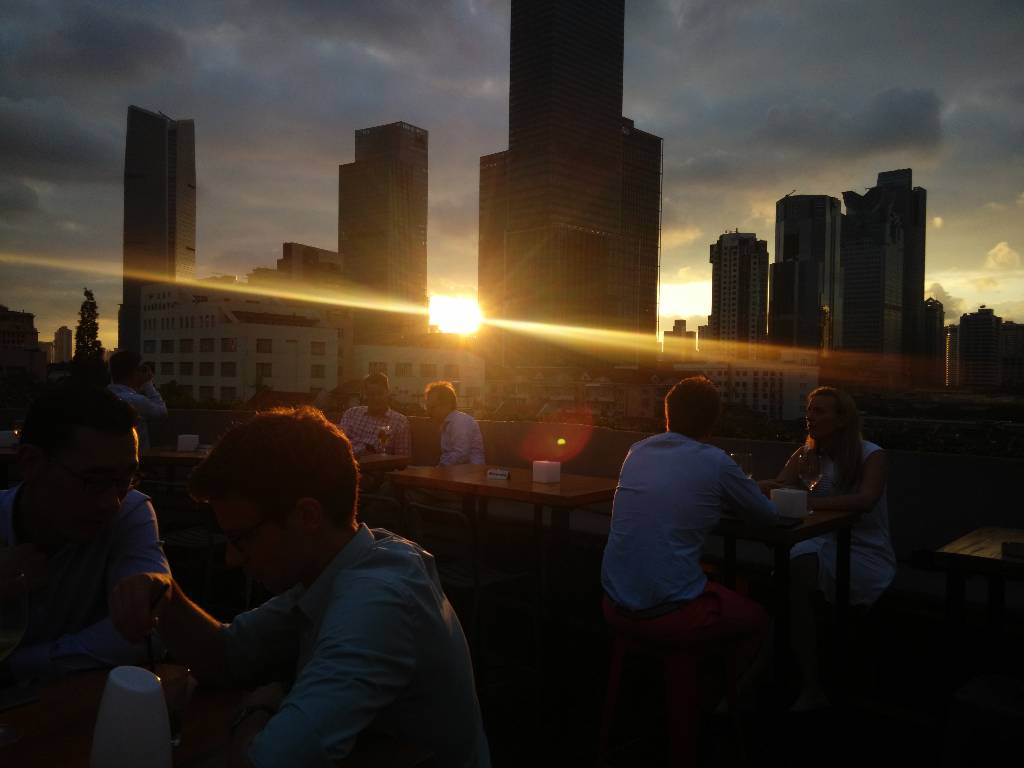
\includegraphics[width=0.95\textwidth]{photo.jpg}
\end{minipage}
\end{center}
\vfill
% Add a romantic poem at the bottom
\begin{minipage}[r]{0.95\textwidth}
    \linespread{2.0}
\raggedleft
\em
\ClosingPoem
\end{minipage}
    
\end{document}
